% Created 2019-02-13 Wed 14:40
% Intended LaTeX compiler: pdflatex
\documentclass[onecolumn]{amsart}
\usepackage[utf8]{inputenc}
\usepackage[T1]{fontenc}
\usepackage{graphicx}
\usepackage{grffile}
\usepackage{longtable}
\usepackage{wrapfig}
\usepackage{rotating}
\usepackage[normalem]{ulem}
\usepackage{amsmath}
\usepackage{textcomp}
\usepackage{amssymb}
\usepackage{capt-of}
\usepackage{hyperref}
                  \usepackage[hyperref,x11names]{xcolor}
\usepackage{hyperref}
\hypersetup{colorlinks=true,citecolor=blue,urlcolor=SteelBlue4,linkcolor=SteelBlue4}
\usepackage{cleveref}
\usepackage{tikz}
\newcommand*\Diff[1]{\mathop{}\!\mathrm{d^#1}}
\usepackage{subcaption}
\author{Rico A.R. Picone}
\date{\today}
\title{Report on spin simulation validation through Gaussian diffusion}
\hypersetup{
 pdfauthor={Rico A.R. Picone},
 pdftitle={Report on spin simulation validation through Gaussian diffusion},
 pdfkeywords={},
 pdfsubject={},
 pdfcreator={rico},
 pdflang={English}}
\begin{document}

\maketitle
\begin{abstract}
A validation test of the \emph{spin transport} software's diffusion behavior is developed and applied.
The validation successfully demonstrates proper diffusion and can now serve as a unit test for future simulation development.
\end{abstract}

\section{Introduction}
\label{sec:org54ab8da}
The bulk spin transport equations include both \emph{diffusion} and \emph{separation} terms.
The separation terms emerge from inter-species interaction through the dipole energy density.
If the separation terms are excluded, the intra-species dynamics should be simply diffusive with known diffusion rates.
For certain initial conditions, the distribution shapes that emerge from this diffusion are predictable and serve as good unit tests for simulation validation.

\section{Gaussian diffusion}
\label{sec:org05792ba}
Excluding separative terms, the spin transport equation for each species's polarization (nuclear or electron) becomes\footnote{For simplicity, we are using \(\rho_i\) for either nuclear (\(i=2\)) or electron (\(i=3\)) polarization, \(\overline{r}\) for the dimensionless spatial coordinate, \(\overline{t}\) for dimensionless time, and \(\overline{\Gamma}_i\) for either species's dimensionless diffusion rate constant. By definition, \(\overline{\Gamma}_2 = 1\) and from the ratio for the simulation species, \(\overline{\Gamma}_3 = 22.335 \cdot 10^{3}\). See \cite{Picone2014b,Picone2019} for detailed variable definitions.}

\begin{equation}
\label{eq:diffusion}
\partial_{\overline{t}} \rho_i(\overline{t},\overline{r}) =
\overline{\Gamma}_i \partial_{\overline{r}^2} \rho_i(\overline{t},\overline{r}).
\end{equation}

\Cref{eq:diffusion} has the well-known Gauss-Weierstrass integral solution \cite{merryfield2009}
\begin{equation}
\label{eq:solution}
\rho_i(\overline{t},\overline{r}) =
\frac{1}{\sqrt{4\pi \overline{t}}}
\int_{-\infty}^\infty f(x) \exp\!\left(-\frac{(\overline{r}-x)^2}{4 \overline{\Gamma}_i \overline{t}}\right) \mathrm{d}x
\end{equation}
where \(f\) is the initial condition \(f(\overline{r}) = \rho_i(0,\overline{r})\).
If we let the initial condition be a Dirac delta function \(f(\overline{r}) = \delta(\overline{r})\), its sifting property yields the solution
\begin{equation}
\label{eq:solution-dirac}
\rho_i(\overline{t},\overline{r}) =
\frac{1}{\sqrt{4\pi \overline{\Gamma}_i \overline{t}}}
\exp\!\left(-\frac{\overline{r}^2}{4 \overline{\Gamma}_i \overline{t}}\right).
\end{equation}
So with an initial Dirac delta polarization distribution, the response of each polarization \(\rho_i\) should be Gaussian.

\section{Simulation and fitting}
\label{sec:org795705d}
In the following, the bulk transport equations are simulated with the \emph{spin transport} software \cite{Picone2019}.\footnote{The results that follow are from the MATLAB version of the software, given here: \url{https://github.com/ricopicone/spin-transport-matlab}.}
The simulation is specifically for the transport equations without separative terms, à la \Cref{eq:diffusion}.
Each nuclear and electron polarization initial conditions are defined to be narrow Gaussian distributions with peaks at unity polarization.
This approximates the Dirac delta initial condition used to derive \Cref{eq:solution-dirac}.
The simulation results are presented in \Cref{fig:1}.
As we expect, Gaussian-like profiles are observed to develop in both species, but they progress at significantly different rates.

\begin{figure}
\begin{subfigure}[b]{.5\linewidth}
\centering
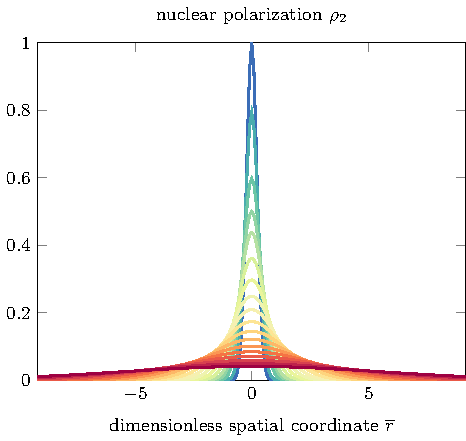
\includegraphics[width=.95\linewidth]{figures/rho_2_snapshots_standalone.pdf}
\caption{\small $\rho_2$ diffusion for $\overline{t} \in 0$\,
\includegraphics[height=1.5ex,width=.5in]{figures/colorbar.pdf}\,$15$.}\label{fig:1a}
\end{subfigure}%
\begin{subfigure}[b]{.5\linewidth}
\centering
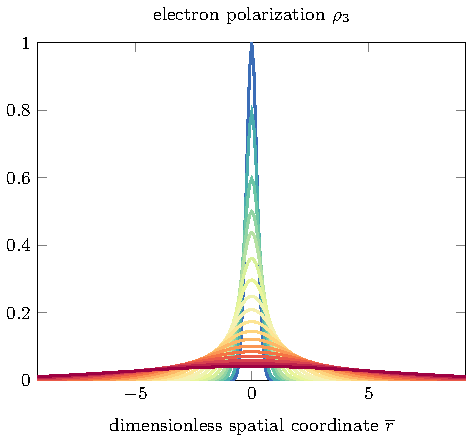
\includegraphics[width=.95\linewidth]{figures/rho_3_snapshots_standalone.pdf}
\caption{\small $\rho_3$ diffusion for $\overline{t} \in 0$ \,
\includegraphics[height=1.5ex,width=.5in]{figures/colorbar.pdf}\,$6.8\cdot 10^{-4}$.}\label{fig:1b}
\end{subfigure}
\caption{Nuclear and electron polarization diffusion profiles through time. The profiles appear identical, but occur at significantly different rates. The electron diffusion occurs at a rate $\overline{\Gamma}_3/\overline{\Gamma}_2$ faster than nuclear diffusion.}\label{fig:1}
\end{figure}

The rates at which the Gaussian width increases is governed by the denominator of the exponential in \Cref{eq:solution-dirac}.
At each moment in simulation time, a Gaussian was curve-fit to each polarization distribution.
Specifically, the parameters estimated were \(a\), \(b\), and \(c\) in the following expression:
\begin{align}
a \exp\!\left(
-\frac{(\overline{r}-b)^2}{c^2}
\right).
\end{align}
Comparing this expression to \Cref{eq:solution-dirac} reveals that, assuming a good Gaussian fit,
\begin{align}
c^2/4 = \overline{\Gamma}_i \overline{t}.
\end{align}
Therefore, the estimate \(c^2/4\) should be approximately linear through time with slope \(\overline{\Gamma}_i\).
That is, the polarization should be Gaussian with variance \(\overline{\Gamma}_i \overline{t}\).

\begin{figure}
\begin{subfigure}[b]{.5\linewidth}
\centering
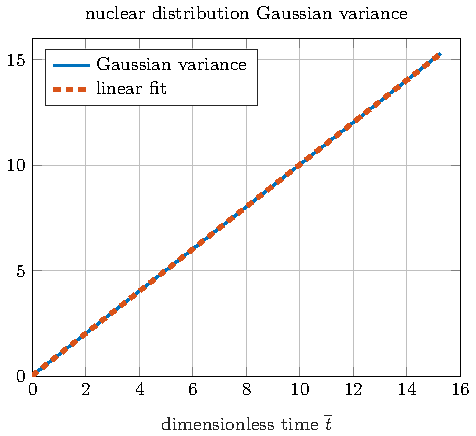
\includegraphics[width=.95\linewidth]{figures/gaussian_variance_vs_time_2_standalone.pdf}
\caption{\small $\rho_2$ Gaussian variance through time in \newline agreement with predicted slope $\overline{\Gamma}_2 = 1$.}\label{fig:2a}
\end{subfigure}%
\begin{subfigure}[b]{.5\linewidth}
\centering
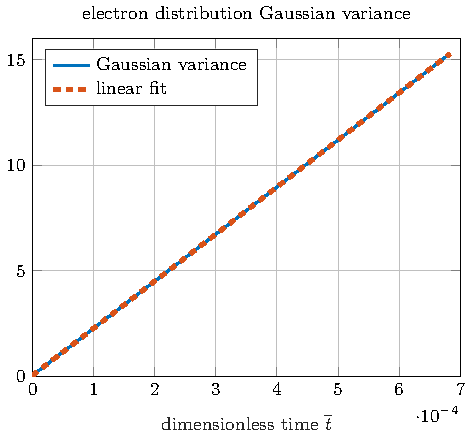
\includegraphics[width=.95\linewidth]{figures/gaussian_variance_vs_time_3_standalone.pdf}
\caption{\small $\rho_3$ Gaussian variance through time in \newline agreement with predicted slope $\overline{\Gamma}_3 = 22 \cdot 10^{3}$.}\label{fig:2b}
\end{subfigure}
\caption{Nuclear and electron Gaussian variances through time, estimated by curve-fitting the spatial distributions of polarization at each moment in simulation-time.}\label{fig:2}
\end{figure}

\Cref{fig:2} shows excellent agreement between the predicted linearity of the Gaussian variance and the simulation results.
The results are not only linear, their slopes are in agreement with the predicted slopes of \(\overline{\Gamma}_2 = 1\) and \(\overline{\Gamma}_3 = 22.3\cdot 10^3\).

\section{Conclusions}
\label{sec:org6d61818}

The simulation is in excellent agreement with the predicted linearity of the Gaussian variance through time.
This validates that the simulation is operational in its diffusivity.
This test can now be added to a suite of automatic unit tests for the \emph{spin transport} software.

\bibliographystyle{unsrt}
\bibliography{report_01}
\end{document}
